\section{Our computational model of serendipity} \label{sec:our-model}

Figure \ref{fig:model} recapitulates the ideas from the previous
section, integrating them into a computationally meaningful model of
process.  The model is summarised in text form at the end of this
section, in our working definition of serendipity.

Figure \ref{fig:1a} is a heuristic map of the features of serendipity
introduced in Section \ref{sec:by-example}.
%
Dashed paths ending in `\ymark' show some of the things that can go
wrong.  A serendipity trigger might not arise, or might not attract
interest.  If interest is aroused, a path to a useful result may not
be sought, or may not be found.  If a result is
developed, it may turn out to be of little value.  Prior experience
with a related problem could be informative, but could also hamper
innovation.  Similarly, multiple tasks, influences, and
contexts can help to foster an inventive frame of mind, but they may
also be distractions.

Figure \ref{fig:1b} removes these unserendipitous paths to focus on
the key features of ``successful'' serendipity.
%
The \textbf{serendipity trigger} is denoted here by $T$.  
%
The \textbf{prepared mind} corresponds to those preparations, labeled
$p$ and $p^{\prime}$, that are relevant to the discovery and invention
phases, respectively.  These preparations may include training,
current attitude, access to relevant knowledge sources, and so on.
%
A \textbf{focus shift} takes place when the trigger is observed to be
interesting.  The now-interesting trigger is denoted $T^\star$, and is
common to both the discovery and the invention phases.
%
%
The \textbf{bridge} is comprised of the actions based on $p^{\prime}$
that are taken on $T^\star$ leading to the \textbf{result} $R$, which is ultimately given a positive evaluation.

\afterpage{\clearpage}
\begin{figure}[p]
\vspace{2mm}
\begin{minipage}[b]{\textwidth}
{\centering
\resizebox{1.02\textwidth}{!}{
\begin{tikzonimage}[width=.45\textwidth,angle=270]{figures/model-diagram/serendipity-attractor-bw}%[tsx/show help lines]
\node (dynamic)[rotate=90] at (-.02, .25) {\emph{dynamic world}};
\node (trigger) at (.05, .255) {\textbf{trigger}};
\node (chance) at (.045, .165) {chance};
\node (bridge) at (.46, .83) {\textbf{bridge}};
\node (result) at (.055, .665) {\textbf{result}};
\node (result)[text width=2cm,align=center] at (.7, .71) {\textbf{prepared mind}};
\node (focus) at (.95, .86) {{\bf \textsc{focus shift}}};
\node (curiosity)[rotate=35] at (.44,.58) {curiosity};
\node (sagacity)[rotate=-30] at (.72,.45) {sagacity};
\node (value) at (.04, .77) {value};
\node (influences)[text width=2cm,align=center,rotate=30] at (.99, .60) {{\small\baselineskip=2pt \emph{multiple influences}\par}};
\node (tasks)[text width=1.5cm,align=center,rotate=30] at (.85, .39) {{\small\baselineskip=2pt \emph{multiple tasks}\par}};
\node (contexts)[text width=1.5cm,align=center,rotate=30] at (.545, .47) {{\small\baselineskip=2pt \emph{multiple contexts}\par}};
\draw[-latex] (.05,.03) -- (.15,.03) node [midway, above] {\itshape{\scshape{discovery}}};
\draw[-latex] (.95,.03) -- (.85,.03) node [midway, above] {\itshape{\scshape{invention}}};
%% Adding an arrowhead
\draw[-{Latex[width=2mm]}] (-.001,.6265) -- (-.003,.6265);
% \node (begin1) at (-.02,.303) {\handmark};
\node (yes1) at (-.02,.6265) {\sunmark};
\node (no1) at (1.005, .165) {\ymark};
\node (no2) at (1.005, .3) {\ymark};
\node (no3) at (.63, .32) {\ymark};
\node (no4) at (0.003, .525) {\ymark};
\end{tikzonimage}

}


\par}
\vspace{-4mm}
\subcaption{A heuristic map, showing serendipitous and unserendipitous outcomes}\label{fig:1a}
\end{minipage}
\medskip

%%%%%%%%%%%%%%%%%%%%%%%%%%%%%%%%%%%%%%%%%%%%%%%%%%%%%%%%%%%%%%%%%%%%%%%%%%%%%%%%%%%%%%%%%%%%%%%%%%%%
\begin{minipage}[b]{\textwidth}
{\centering
\begingroup
\tikzset{
block/.style = {draw, fill=white, rectangle, minimum height=3em, minimum width=3em},
tmp/.style  = {coordinate}, 
sum/.style= {draw, fill=white, circle, node distance=1cm},
input/.style = {coordinate},
output/.style= {coordinate},
pinstyle/.style = {pin edge={to-,thin,black}}
}

\begin{tikzpicture}[auto, node distance=2cm,>=latex']
    \node [sum] (sum1) {};
    \node [input, name=pinput, above left=.7cm and .7cm of sum1] (pinput) {};
    \node [input, name=tinput, left of=sum1] (tinput) {};
    \node [input, name=minput, below left of=sum1] (minput) {};
    \node [input, name=minput, right of=sum1] (moutput) {};
    \draw [->] (pinput) -- node{$p$} (sum1);
    \draw [->] (tinput) -- node{\vphantom{{\tiny g}}$T$} (sum1);
    \draw [->] (sum1) -- node{\vphantom{{\tiny g}}$T^{\star}$}  (moutput);
\end{tikzpicture}
\hspace{1cm}
\begin{tikzpicture}[auto, node distance=2cm,>=latex']
    \node [sum] (sum1) {};
    \node [input, name=pinput, above left=.7cm and .7cm of sum1] (pinput) {};
    \node [input, name=tinput, left of=sum1] (tinput) {};
    \node [input, name=minput, below left of=sum1] (minput) {};
    \node [sum, right of=sum1] (sum2) {};
    \node [input, name=minput, right of=sum2] (moutput) {};
    \draw [->] (pinput) -- node{$p^{\prime}$} (sum1);
    \draw [->] (tinput) -- node{\vphantom{{\tiny g}}$T^{\star}$} (sum1);
    \draw [->] (sum1) -- node{\vphantom{{\tiny g}}$R$} (sum2);
    \draw [->] (sum2) -- node{$|R|>0$}  (moutput);
\end{tikzpicture}
\endgroup


%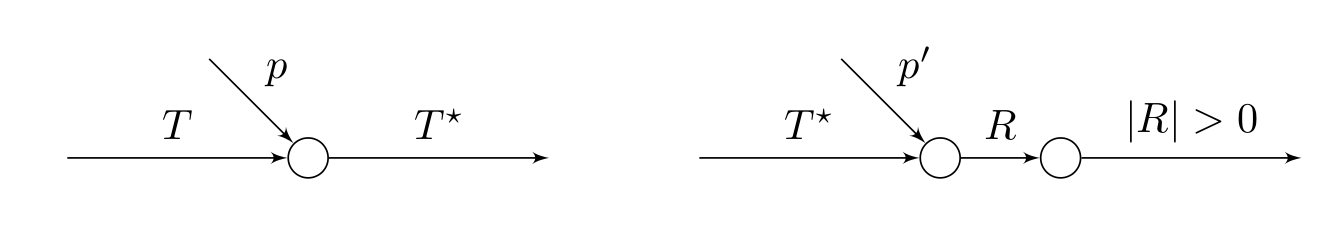
\includegraphics[width=.8\textwidth]{schematic}
\par}
\subcaption{A simplified process schematic, showing the key features of the model}\label{fig:1b}
\end{minipage}
\medskip

%%%%%%%%%%%%%%%%%%%%%%%%%%%%%%%%%%%%%%%%%%%%%%%%%%%%%%%%%%%%%%%%%%%%%%%%%%%%%%%%%%%%%%%%%%%%%%%%%%%%
\begin{minipage}[b]{\textwidth}
{\centering
\begin{tikzpicture}[
single/.style={draw, anchor=text, rectangle},
]
\node (discovery) {\textbf{\emph{Discovery:}}};
% poet generates poem
\node[single, right=8mm of discovery.east,text width=1.5cm] (poet) {\emph{poetry generator}};
\node[single, right=4mm of poet.east] (poem) {P};
\draw [-latex] (poet.east) -- (poem.west);
% critic listens to poem and offers feedback
\node[single, right=4mm of poem.east,text width=1.5cm] (critic) {comment generator};
\draw [-latex] (poem.east) -- (critic.west);
\node[single, right=4mm of critic.east] (feedback) {F};
\draw [-latex] (critic.east) -- (feedback.west);

%%% Next phase
\node[below=1cm of discovery] (invention) {\textbf{\emph{Invention:}}};
% poet integrates feedback
\node[single, right=8mm of invention.east] (feedbackcont) {F};
\node[single, right=8mm of feedbackcont.east,text width=1.7cm] (integrator) {\emph{feedback integrator}};
\draw [-latex] (feedbackcont.east) -- (integrator.west);

\node[single, below=8mm of integrator.south,text width=1.5cm] (explainer) {feedback explainer};

\node[single, below right=2mm and 2mm of integrator] (question) {Q};
\node[single, below left=2mm and 2mm of integrator] (answer) {A};

\draw[-latex] ([yshift=-1.5mm]integrator.east) to [out=0,in=90] (question.north) ;
\draw[-latex] (question.south) to [out=270,in=0] (explainer.east) ;
\draw[-latex] (explainer.west) to [out=180,in=270] (answer.south) ;
\draw[-latex] (answer.north) to [out=90,in=180] ([yshift=-1.5mm]integrator.west) ;

\node[single, right=8mm of integrator.east] (problem) {X};

\draw [-latex] (integrator.east) -- (problem.west);

% poet reflects on feedback and updates codebase

\node[single, right=4mm of problem.east,text width=1.5cm] (pgrammer) {\emph{code}\\ \emph{generator}};

\draw [-latex] (problem.east) -- (pgrammer.west);

\node[single, right=4mm of pgrammer.east,text width=.3cm] (etc) {...};

\draw [-latex] (pgrammer.east) -- (etc.west);
\end{tikzpicture}

%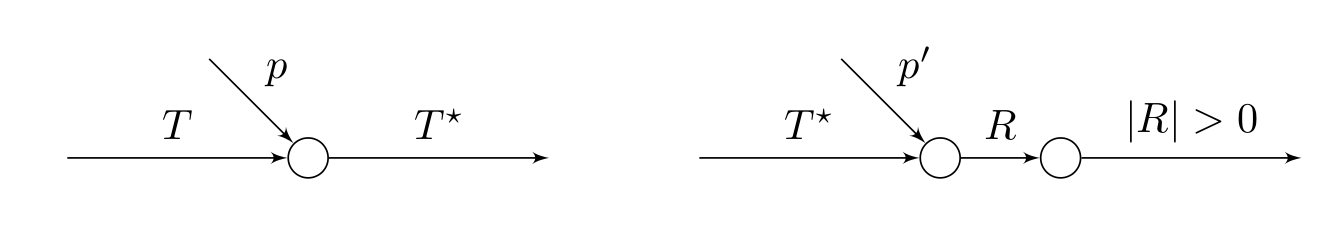
\includegraphics[width=.8\textwidth]{schematic}

\par}
\smallskip

\subcaption{A boxes-and-arrows diagram, showing one possible implementation architecture}\label{fig:1c}
\end{minipage}
\bigskip

\caption{Three representations of the elements of serendipity}\label{fig:model}
\end{figure}

Figure \ref{fig:1c} expands this schematic into a sketch of the
components of one possible idealised implementation of a serendipitous
system.  An existing \emph{generative process} is assumed.  This may
be based on observations of the outside world, or it may be a purely
computational process.  In any case, its products are passed on to the
next stage.  After running this data through a feedback loop, certain
aspects of the data are singled out, and marked up as
``interesting.''  Note that this designation need not arise all at
once: rather, it the outcome of a \emph{reflective process}.  In the
implementation envisioned here, this process makes use of two primary
functions: $p_1$, which notices particular aspects of the data, and $p_2$, which
offers reflections about those aspects.  Together, these functions build up a
``feedback object,'' $T^{\star}$, which consists of the original data
and further metadata.  This is passed on to an \emph{experimental
  process}, which has the task of verifying that the data
is indeed interesting, and determining what it may be useful for.
This is again an iterative process, relying on functions $p^{\prime}_1$ and $p^{\prime}_2$, which
build a contextual understanding of the trigger by devising experiments and
assessing their results.  Once implications or applications have been found, a result is
generated, which is passed to a final \emph{evaluation process}, and,
from there, to applications.

The ellipses at the end of the workflow in Figure \ref{fig:1c} are
intended to suggest that applications are open-ended; however, an
important class of applications will result in changes to one or more
of the system's modules, for example by expanding the knowledge base
that they have available.  Note that earlier components of the workflow
cannot, in general, anticipate what the subsequent phases will produce
or achieve.  If the system's next steps could be anticipated, we would
not say that the behaviour was serendipitous.  In other words,
serendipity does not adhere to one specific part of the system, but to
its operations as a whole.  Although Figures  \ref{fig:1b} and  \ref{fig:1c}
treat the case of successful serendipity, as indicated in Figure
 \ref{fig:1a}, each step is fallible, as is the system as a whole.
Thus, for example, a trigger that has been initially tagged as interesting may prove to be fruitless.
Similarly a system that implements all of the steps in Figure \ref{fig:1c}, but that never
achieves results of value does not have potential for serendipity.
However, a system only produces results of high value would also be
suspect, since it would indicate a tight coupling between trigger
and outcome.  Fallibility is a ``meta-criterion'' that transcends the criteria from Section \ref{sec:by-example}.
Summarising, we propose the following:
\begin{ndef}
\emph{(1) Within a system with a prepared mind, a previously uninteresting serendipity trigger arises due to circumstances that the system does not control and cannot predict, and is classified as interesting by the system; and,}
\emph{(2) The system uses the trigger and prior preparation, together with relevant computational processing, networking, and experimental techniques, to obtain a novel result that is evaluated favourably by the system or by external sources.}
\end{ndef}


